Quando o objetivo central de uma pesquisa é construir e avaliar um artefato computacional — e não apenas observar ou descrever um fenômeno —, a escolha metodológica deve refletir essa natureza construtiva. É nesse sentido que se adota o \textit{Design Science Research} (DSR), um paradigma consolidado em Ciência da Computação que orienta não apenas a construção do artefato, mas a geração de conhecimento científico a partir do processo de design, implementação e avaliação \cite{Peffers2007}. O risco de trabalhos dessa natureza é reduzir-se a um relatório técnico de desenvolvimento de software; a DSR evita isso ao exigir que cada decisão de design seja justificada teoricamente e que os resultados sejam avaliados com rigor comparável ao de pesquisas empíricas \cite{Runeson2020, Pimentel2020}. As seis fases que estruturam esta pesquisa são descritas a seguir.

\section{Abordagem Metodológica: Design Science Research}

A metodologia foi estruturada seguindo o ciclo de processo proposto por Peffers et al. \cite{Peffers2007}, adaptado para o contexto deste trabalho em seis fases principais, conforme ilustrado na Figura \ref{fig:fluxo_trabalho_projeto}:

\begin{enumerate}
    \item Identificação do Problema e Motivação
    \item Definição dos Objetivos da Solução
    \item Design e Desenvolvimento do Artefato
    \item Demonstração
    \item Avaliação
    \item Reflexão e Aprendizados
\end{enumerate}

\begin{figure}[H]
    \centering
    \caption{Fluxo metodológico baseado em Design Science Research (adaptado de Peffers et al. 2007)}
    \label{fig:fluxo_trabalho_projeto}
    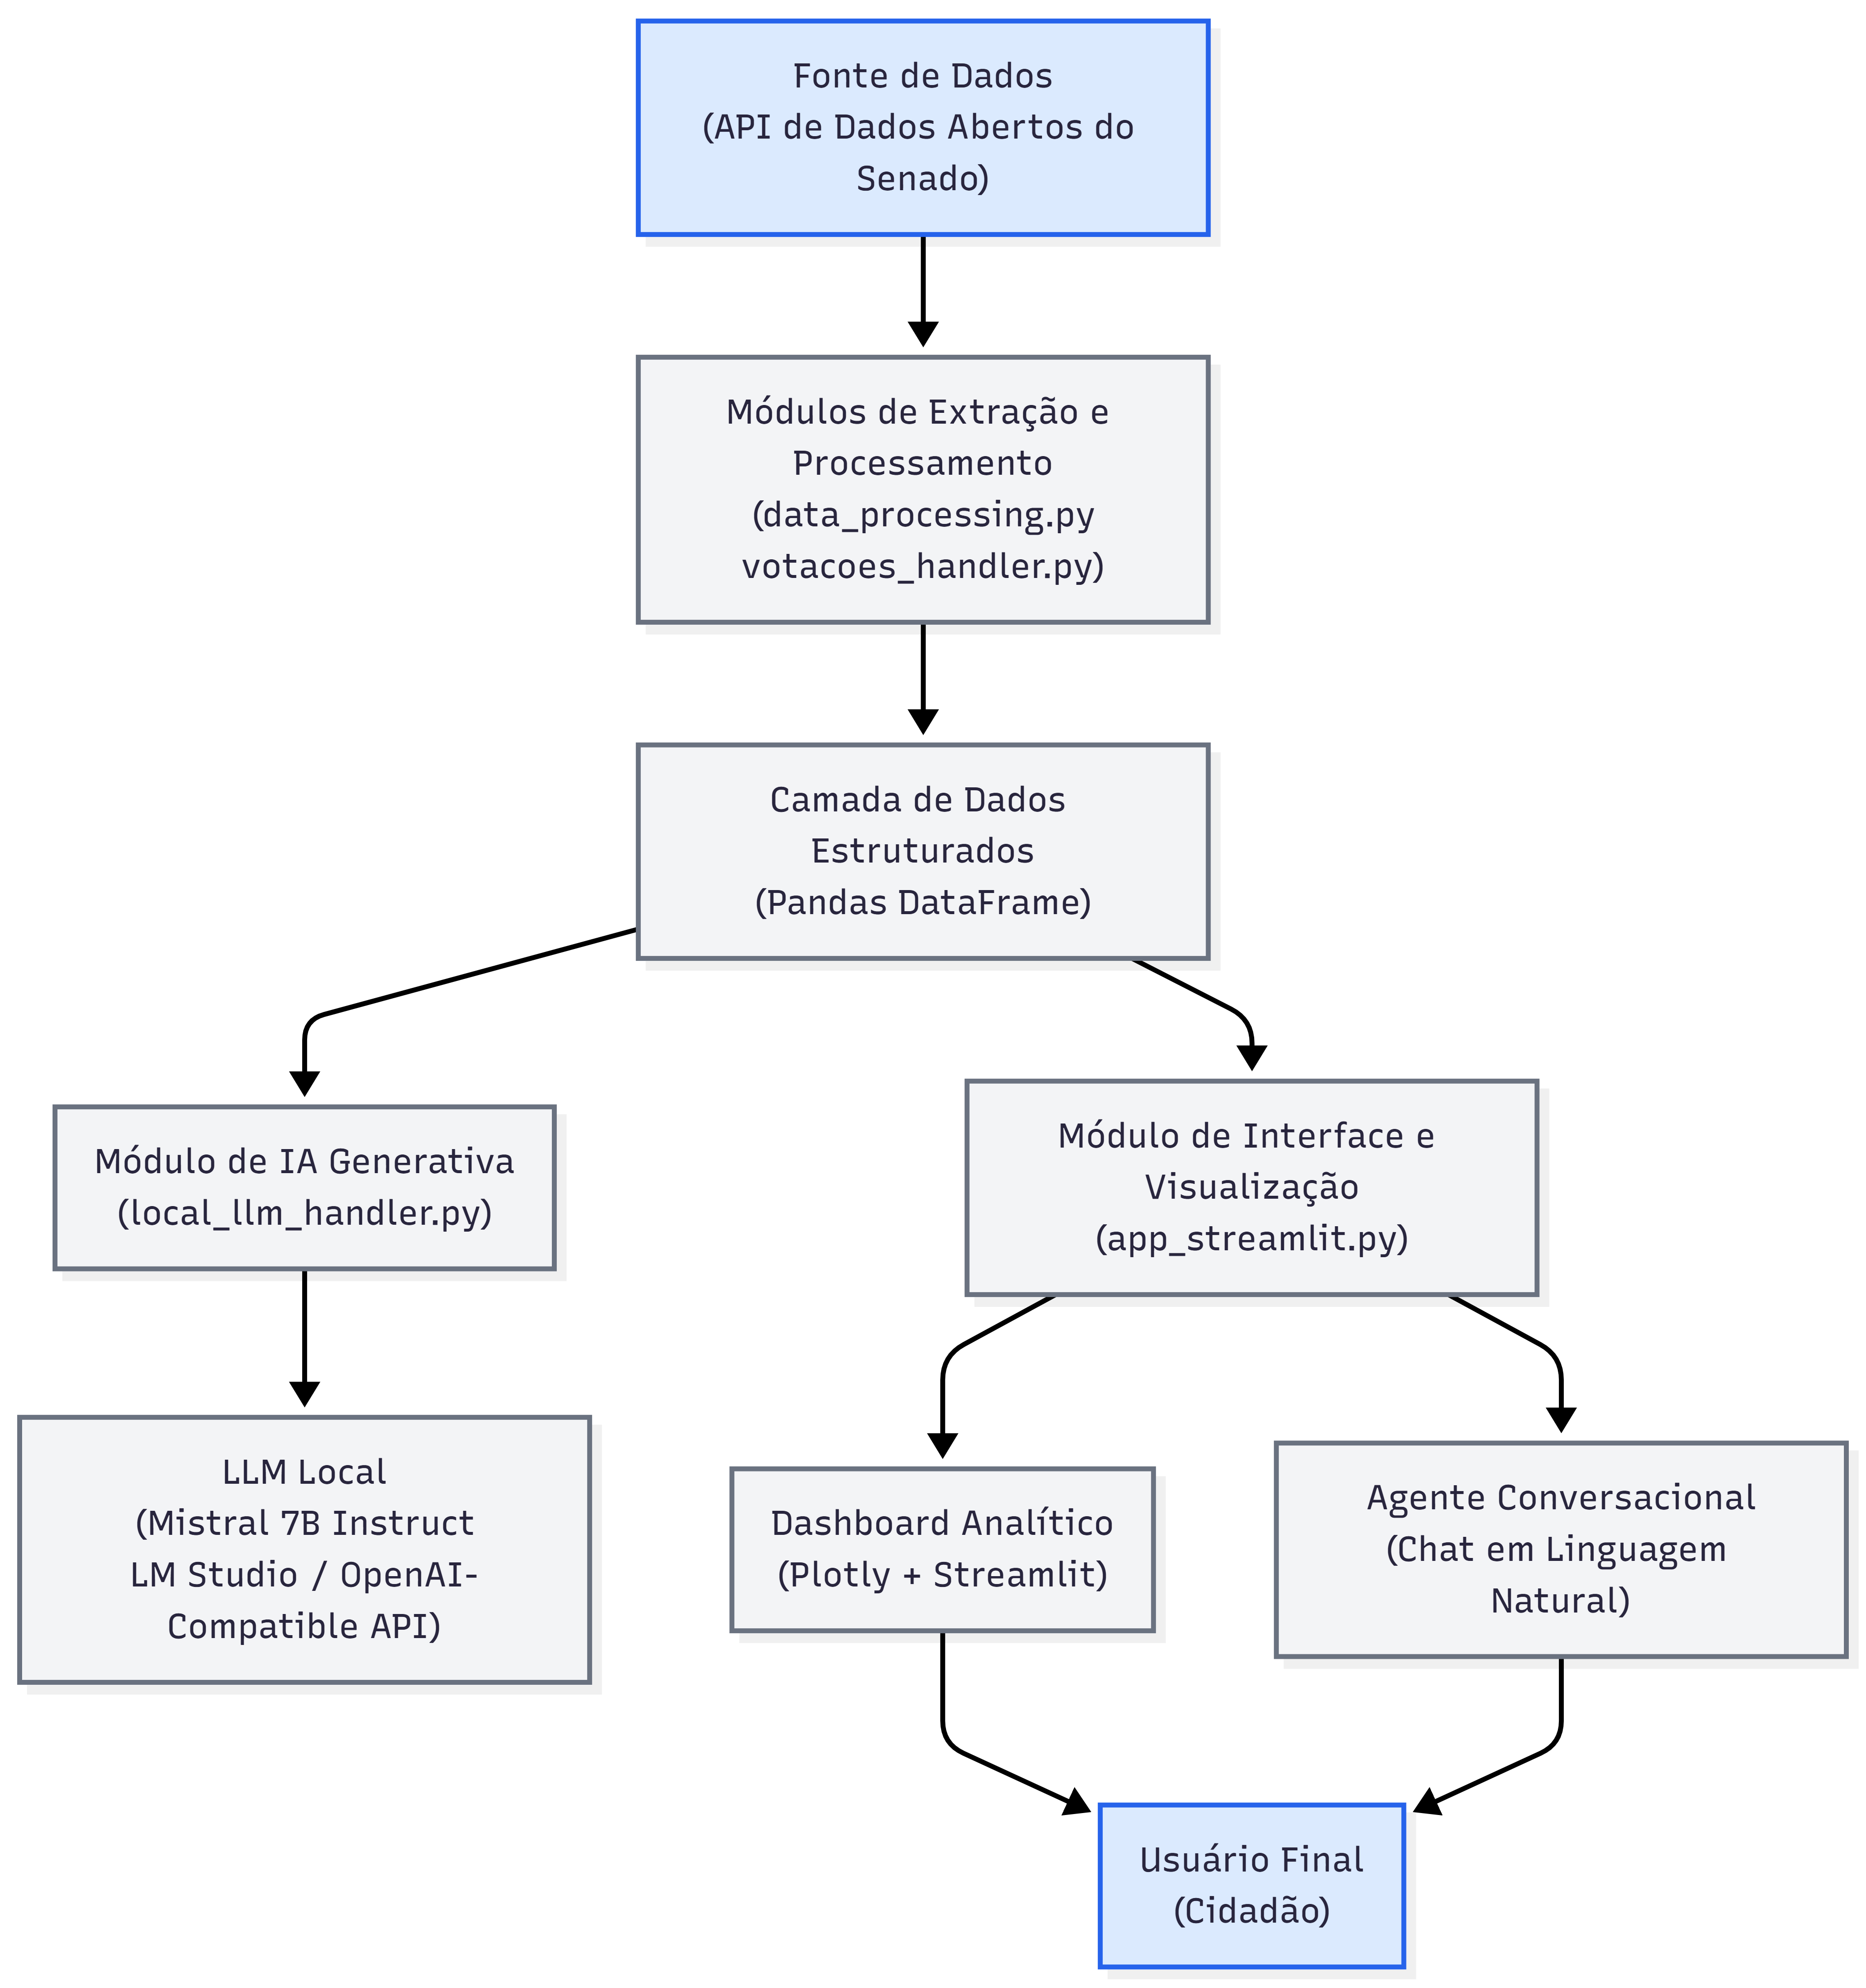
\includegraphics[width=0.8\textwidth]{imagens/fluxo_trabalho_projeto.png}
    \fonte{Adaptado de Peffers et al. (2007).}
\end{figure}

\section{Fases da Pesquisa}

\subsection{Fase 1: Identificação do Problema e Motivação}

A primeira etapa consistiu no reconhecimento da opacidade prática dos dados parlamentares. Embora disponíveis em formato aberto através da API do Senado Federal, a complexidade técnica e o volume massivo desses dados impedem que cidadãos comuns exerçam controle social efetivo. Segundo Oliveira e Ckagnazaroff \cite{OliveiraCkagnazaroff2022}, para que a transparência seja efetiva, os dados devem ser não apenas públicos, mas também claros, contextualizados e utilizáveis.

Conforme apontado por Lee et al. \cite{Lee2017} através do VLAT, nem todos conseguem interpretar visualizações gráficas complexas. Complementarmente, Hornung et al. \cite{Hornung2015} demonstram que usuários sem formação estatística frequentemente não conseguem analisar dados de forma autônoma. Consequentemente, a mera disponibilização de dados não garante compreensão ou participação democrática.

Esta fase foi fundamentada em revisão de literatura e análise exploratória da API do Senado Federal, identificando-se a lacuna entre disponibilidade técnica de dados e acessibilidade cognitiva para cidadãos.

\subsection{Fase 2: Definição dos Objetivos da Solução}

Definiu-se que o artefato a ser construído deveria reduzir as barreiras cognitivas de acesso aos dados parlamentares. Para isso, estabeleceu-se que a solução deveria:

\begin{enumerate}
    \item \textbf{Automatizar a extração de dados brutos:} Implementar pipeline de ETL para processar dados da API do Senado, convertendo formatos não estruturados (XML/JSON) em estruturas tabulares otimizadas para análise.

    \item \textbf{Traduzir linguagem parlamentar:} Utilizar IA Generativa para categorizar e resumir discursos parlamentares complexos, tornando-os compreensíveis para cidadãos sem expertise na área.

    \item \textbf{Permitir interação em linguagem natural:} Implementar interface conversacional que permita ao usuário formular perguntas em linguagem comum, dispensando conhecimento técnico de queries ou programação.

    \item \textbf{Oferecer múltiplas modalidades de exploração:} Combinar Dashboard visual (para exploração livre) com Chatbot conversacional (para consultas diretas), atendendo diferentes estilos cognitivos de usuários.
\end{enumerate}

\section{Fase 3: Design e Desenvolvimento do Artefato}

Nesta fase, correspondente à construção técnica da solução, a aplicação foi desenvolvida em Python sob uma arquitetura modular, visando garantir manutenibilidade e escalabilidade. A solução foi segmentada em três camadas principais:

\subsection{Coleta e Processamento de Dados (Camada de Dados)}

A coleta foi efetuada via API de Dados Abertos do Senado Federal \cite{SenadoFederal_s_d}. O processo de ETL (\textit{Extract, Transform, Load}) incluiu:

\begin{itemize}
    \item \textbf{Requisição:} Uso da biblioteca \textit{Requests} \cite{RequestsLib} para extração de dados brutos (XML/JSON) dos \textit{endpoints} mapeados via Swagger (Figura \ref{fig:senado_swagger}).
    \item \textbf{Estruturação:} Conversão e limpeza dos dados utilizando \textit{Pandas} \cite{PandasLib}, organizando discursos e votações em estruturas tabulares otimizadas para análise.
\end{itemize}

\begin{figure}[H]
    \centering
    \caption{Interface Swagger da API de Dados Abertos do Senado Federal}
    \label{fig:senado_swagger}
    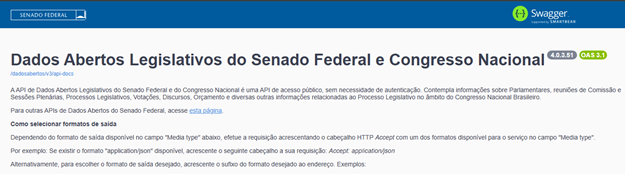
\includegraphics[width=0.9\textwidth]{imagens/senado_swagger.png}
    \fonte{Senado Federal.}
\end{figure}

\subsection{Análise com IA Generativa (Camada de Inteligência)}

O núcleo analítico utiliza o modelo Mistral 7B Instruct \cite{MistralAI2024}, que roda em ambiente local. Diferente de abordagens que dependem de APIs proprietárias, esta etapa emprega engenharia de \textit{prompts} para duas funções críticas:

\begin{itemize}
    \item \textbf{Classificação Temática:} Categorização automática de discursos em temas (ex: "Saúde", "Educação", "Infraestrutura") utilizando \textit{prompts} estruturados e exemplos de Few-Shot Learning.

    \item \textbf{Motor de Resposta (Recuperação Estruturada com Geração Aumentada):} O módulo recebe perguntas do usuário em linguagem natural, recupera da base em memória (cache de sessão) um subconjunto de registros relevantes e instrui o modelo Mistral 7B a gerar respostas contextualizadas e didáticas, compreensíveis para cidadãos não-especialistas, fundamentadas nesses registros e citando-os por identificador estável, de modo a preservar a rastreabilidade entre resposta e dados.
\end{itemize}

A justificativa detalhada para a escolha do Mistral 7B em ambiente local --- replicabilidade, soberania de dados e sustentabilidade operacional ---, bem como a comparação com modelos proprietários e com outros modelos abertos contemporâneos, encontra-se na fundamentação teórica (Seção~\ref{subsec:escolha_modelo}). Aqui interessa registrar apenas que essa decisão de design condiciona o protocolo de avaliação descrito adiante, em especial a comparação da classificação temática com uma linha de base sem LLM.

\subsection{Interface Interativa (Camada de Apresentação)}

Para materializar o acesso democrático aos dados, desenvolveu-se uma interface \textit{web} utilizando o \textit{framework Streamlit} \cite{Streamlit2024}, oferecendo dois modos de interação complementares:

\begin{itemize}
    \item \textbf{\textit{Dashboard} Visual:} Gráficos interativos gerados com \textit{Plotly} \cite{Plotly2024} para exploração de tendências legislativas. O dashboard permite que usuários visualizem panoramicamente os dados, seguindo o princípio de Shneiderman \cite{Shneiderman1996} de "zoom and filter" (Figura \ref{fig:tela_aplicacao}).

    \item \textbf{Agente Conversacional:} Interface de \textit{chat} que abstrai a complexidade dos dados, permitindo consultas diretas em linguagem natural como "Como votou o Senador X sobre educação?" ou "Qual foi o tema mais debatido em 2025?" (Figura \ref{fig:tela_aplicacao}).
\end{itemize}

\begin{figure}[H]
    \centering
    \caption{Interface da Aplicação}
    \label{fig:tela_aplicacao}
    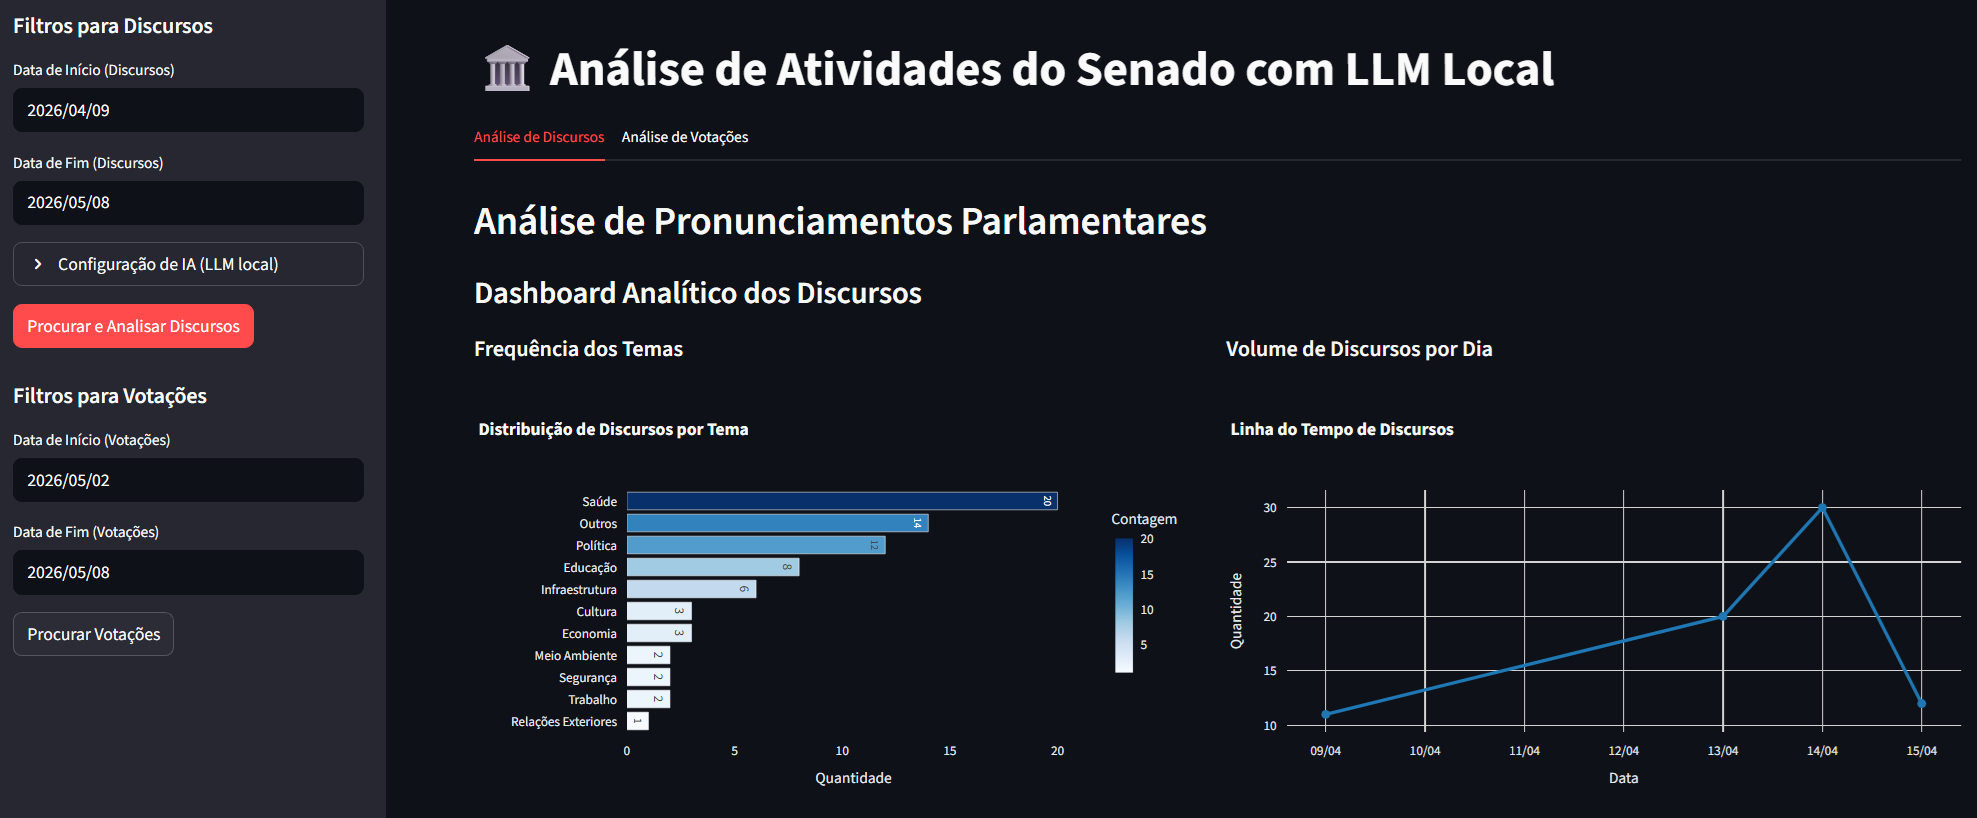
\includegraphics[width=0.9\textwidth]{imagens/tela_aplicacao.png}
    \fonte{Produção da autora.}
\end{figure}

\section{Fundamentos Teóricos para as Escolhas de Design}

A combinação de Dashboard e Chatbot não é arbitrária, mas fundamentada em teorias de Interação Humano-Computador e Acessibilidade de Dados. Esta seção justifica essas escolhas.

\subsection{Por que Dashboard?}

Dashboards e visualizações de dados oferecem exploração livre e visão holística de um corpus de dados. Contudo, conforme Lee et al. \cite{Lee2017} demonstram através do VLAT, nem todos os usuários possuem "visualization literacy" — a capacidade de compreender visualizações gráficas complexas.

Apesar dessa limitação, os \textit{dashboards} oferecem benefícios concretos: permitem ao usuário obter uma visão panorâmica dos dados antes de descer ao detalhe --- seguindo o princípio de Shneiderman \cite{Shneiderman1996} ---, explorar o corpus de forma autônoma e sem intermediário, identificar padrões visuais como tendências e anomalias e, ainda, filtrar e segmentar a informação interativamente. Por isso, o \textit{dashboard} proposto adota decisões de design voltadas à acessibilidade: paleta de cores intuitiva, títulos e rótulos em linguagem comum em vez de jargão legislativo, preferência por representações simples --- barras e linhas --- em detrimento de \textit{heatmaps} ou \textit{scatter plots}, e interatividade básica baseada em filtros e em detalhamento sob demanda.

\subsection{Por que Chatbot?}

Interfaces conversacionais, especialmente aquelas alimentadas por Modelos de Linguagem Generativa, reduzem significativamente a barreira de entrada cognitiva. Um usuário sem expertise estatística pode formular perguntas em linguagem natural em vez de construir queries SQL ou manipular dados brutos.

Conforme a pesquisa em Interação Humano-Computador e Interação Humano-Dados \cite{Hornung2015, Brito2024}, as interfaces conversacionais reduzem a barreira de entrada --- o usuário não precisa conhecer a estrutura dos dados nem uma linguagem de consulta ---, apoiam-se em um formato de interação familiar, acomodam formulações distintas para uma mesma necessidade de informação e podem mediar a compreensão, traduzindo resultados técnicos em explicações acessíveis.

Essas vantagens convivem com limitações conhecidas dos \textit{chatbots} baseados em LLMs, sobretudo o risco de alucinação (respostas factualmente incorretas) e a opacidade do processo de geração. Para mitigá-las, a implementação proposta utiliza o Mistral 7B Instruct \cite{Jiang2023}, cujo porte paramétrico reduz a incidência de alucinações em relação a modelos de menor escala; valida as respostas contra os dados reais; e --- ponto central deste trabalho --- garante rastreabilidade, pois o agente recupera um subconjunto de registros da base, cita-os na resposta por identificador estável e expõe, na interface, o painel de fontes utilizadas.

\subsection{Complementaridade: Dashboard + Chatbot}

A literatura em Interação Humano-Dados distingue dois padrões primários de uso em sistemas de informação pública: a exploração orientada à descoberta, em que o usuário navega pelo corpus sem uma pergunta pré-definida, e a consulta orientada a objetivos, em que há uma pergunta específica a ser respondida \cite{Shneiderman1996}. Esses padrões raramente são atendidos com igual eficácia por uma única modalidade de interface.

O \textit{Dashboard} atende principalmente o primeiro padrão: permite ao usuário identificar tendências, comparar parlamentares e detectar anomalias por navegação visual, sem exigir que ele formule uma pergunta antes de começar. O \textit{Chatbot}, por sua vez, é mais adequado ao segundo padrão: reduz a carga cognitiva de quem sabe o que quer perguntar mas não sabe como navegar em dados estruturados. A integração de ambos em um único sistema não busca cobrir todos os perfis de usuário possíveis — uma afirmação que exigiria validação empírica — mas reconhece que restringir a interação a uma única modalidade excluiria sistematicamente parte dos potenciais usuários. Essa decisão de design será discutida nas considerações finais à luz dos resultados da avaliação.

\section{Fase 4: Demonstração}

Em DSR, a Demonstração distingue-se da Avaliação: enquanto esta confronta o artefato com critérios pré-definidos, aquela evidencia a viabilidade do artefato em uso, por meio de ao menos um cenário representativo documentado de ponta a ponta. Nesta fase, o AgentAI foi colocado em ambiente de homologação, processando dados reais da API do Senado Federal, e sua operação foi demonstrada em um fluxo completo: a partir de uma pergunta em linguagem natural (entrada), o sistema recupera os registros pertinentes da base (processamento), gera uma resposta fundamentada (saída) e exibe os registros que a embasam (fontes). Esse fluxo abrange o processamento automático de sessões legislativas reais, a classificação temática dos discursos, a resposta a consultas em linguagem natural e a visualização de tendências legislativas, confirmando a viabilidade técnica que habilita a fase de avaliação rigorosa. A verificação funcional preliminar correspondente é reportada no Capítulo~\ref{cap:desenvolvimento}.

\section{Fase 5: Avaliação do Artefato}

A fase de avaliação será conduzida sem entrevistas, questionários, observação comportamental ou qualquer coleta de dados com participantes humanos. A avaliação incidirá sobre o artefato computacional, os dados públicos processados e as respostas geradas pelo modelo. Dessa forma, a pesquisa utiliza exclusivamente dados abertos, informações de domínio público e análises técnicas do sistema.

A avaliação foi organizada em quatro frentes complementares: qualidade da coleta e estruturação dos dados, classificação temática, qualidade factual das respostas e rastreabilidade das informações apresentadas pelo agente conversacional. O Quadro~\ref{quad:matriz_rastreabilidade} explicita o alinhamento entre os objetivos específicos, as frentes de avaliação, as métricas e as cláusulas da hipótese, tornando rastreável a cadeia que liga a questão de pesquisa aos critérios de avaliação.

\begin{quadro}[H]
    \centering
    \caption{Matriz de rastreabilidade entre objetivos, frentes de avaliação, métricas e cláusulas da hipótese}
    \label{quad:matriz_rastreabilidade}
    \resizebox{\textwidth}{!}{%
    \begin{tabular}{|p{4.2cm}|p{3.4cm}|p{5.0cm}|p{2.4cm}|}
        \hline
        \textbf{Objetivo específico} & \textbf{Frente de avaliação} & \textbf{Métricas principais} & \textbf{Cláusula da hipótese} \\
        \hline
        Processar e estruturar os dados da API do Senado & Coleta e estruturação & Completude, consistência, reprodutibilidade & Premissa (estruturar) \\
        \hline
        Classificar tematicamente os discursos & Classificação temática & Acurácia, precisão, revocação e F1 \textit{vs.} \textit{baseline} sem LLM & (a) \\
        \hline
        Responder em linguagem natural sobre os dados & Avaliação factual & \% de respostas corretas/parciais/incorretas \textit{vs.} configuração sem recuperação & (b) \\
        \hline
        Avaliar a rastreabilidade das respostas & Rastreabilidade & Cobertura de recuperação e de citação, precisão e suporte semântico da citação & (c) \\
        \hline
        Consolidar o uso do artefato & Cenários de uso & Síntese qualitativa dos casos de teste & Premissa (consultar) \\
        \hline
    \end{tabular}%
    }
    \fonte{Produção da autora.}
\end{quadro}

\subsection{Avaliação da Coleta e Estruturação dos Dados}

\subsubsection{Pergunta}
Em que medida o pipeline de coleta e processamento estrutura corretamente os dados parlamentares obtidos da API do Senado Federal?

\subsubsection{Método}
Será selecionado um conjunto de endpoints e períodos de coleta definidos no escopo do estudo. Os dados retornados pela API serão comparados com as estruturas armazenadas localmente pelo AgentAI, verificando se os campos essenciais foram preservados e se o processo de transformação não introduziu inconsistências.

\subsubsection{Métricas}
\begin{itemize}
    \item \textbf{Completude:} proporção de registros coletados e armazenados com campos essenciais preenchidos.
    \item \textbf{Consistência:} ausência de duplicidades, datas inválidas, campos incompatíveis ou vínculos incorretos entre parlamentar, discurso, votação e matéria.
    \item \textbf{Reprodutibilidade:} capacidade de reexecutar o pipeline e obter uma base equivalente para o mesmo recorte temporal.
\end{itemize}

\subsection{Avaliação da Classificação Temática}

\subsubsection{Pergunta}
Em que medida o modelo Mistral 7B Instruct classifica corretamente os temas dos discursos parlamentares?

\subsubsection{Método}
As categorias temáticas serão definidas \textit{a priori}, antes de qualquer anotação, a partir das áreas recorrentes na atividade legislativa, fixando-se um número mínimo de instâncias por categoria (ao menos 20) para assegurar a estabilidade das métricas por classe. Sobre essa base, será construída uma amostra de discursos reais do Senado Federal (mínimo de 150 registros, distribuídos entre as categorias) para compor o gabarito de referência. A anotação será realizada de forma independente por dois avaliadores, guiada por um protocolo documentado explicitamente antes do início --- com a definição operacional de cada categoria e exemplos de casos limítrofes. O nível de concordância entre os avaliadores será medido pelo coeficiente Kappa de Cohen \cite{Cohen1960}, adotando-se, antes da anotação, o limiar de concordância substancial ($\kappa \geq 0{,}61$) da escala de Landis e Koch \cite{LandisKoch1977} como critério mínimo aceitável; abaixo desse valor, o protocolo será revisado e a anotação refeita. Para reduzir o risco de viés compartilhado, os casos de discordância remanescentes serão resolvidos por um terceiro anotador independente, e não por discussão entre os dois anotadores iniciais; a concordância será reportada também por classe. A classificação gerada pelo modelo será então comparada com o gabarito final.

\subsubsection{Métricas}
\begin{itemize}
    \item \textbf{Acurácia:} proporção de classificações coincidentes com o gabarito de referência.
    \item \textbf{Precisão:} proporção de discursos classificados em um tema que efetivamente pertencem a esse tema no gabarito.
    \item \textbf{Revocação:} proporção de discursos de um tema que foram corretamente identificados pelo modelo.
    \item \textbf{F1-Score:} média harmônica entre precisão e revocação.
\end{itemize}

\subsubsection{Critério de Interpretação}
Os resultados serão interpretados comparativamente em relação a um \textit{baseline} de referência: uma classificação por correspondência de palavras-chave temáticas predefinidas (abordagem clássica sem LLM). Essa comparação permite dimensionar o ganho — ou ausência de ganho — que o Mistral 7B Instruct oferece em relação a uma solução mais simples. A análise qualitativa complementará os números, identificando os tipos de discurso que geram maior ambiguidade e os casos em que o modelo produz classificações inconsistentes com o gabarito.

\subsection{Avaliação Factual das Respostas do Agente Conversacional}

\subsubsection{Pergunta}
As respostas geradas pelo agente conversacional são coerentes com os dados públicos recuperados da base local?

\subsubsection{Método}
Será elaborado um conjunto de cenários representativos de consulta, definido \textit{a priori} e dimensionado para cobrir todas as classes de pergunta previstas (votações, discursos, parlamentares, temas e períodos) com múltiplas instâncias por classe, totalizando ao menos 30 cenários. Para cada cenário, será definida uma resposta esperada com base nos dados oficiais coletados da API do Senado Federal. As respostas geradas pelo AgentAI serão classificadas em quatro categorias com definição operacional explícita: \textit{correta} (todas as afirmações verificáveis conferem com os dados e nada essencial é omitido); \textit{parcialmente correta} (afirmações corretas convivem com omissões ou imprecisões não centrais); \textit{incorreta} (há ao menos uma afirmação factualmente errada ou sem respaldo nos dados); e \textit{não respondida} (o sistema não responde ou declara não dispor da informação). Para reduzir a subjetividade, a classificação será conduzida por dois avaliadores de forma independente, com a concordância medida pelo Kappa de Cohen \cite{Cohen1960} e as divergências resolvidas por um terceiro avaliador; sempre que a comparação envolver as configurações com e sem recuperação contextual, o avaliador será cegado quanto à origem da resposta. O protocolo será fixado antes da execução.

\subsubsection{Métricas}
\begin{itemize}
    \item Percentual de respostas corretas.
    \item Percentual de respostas parcialmente corretas.
    \item Percentual de respostas incorretas ou sem respaldo nos dados.
    \item Tipos de erro observados, como omissão, generalização indevida, interpretação incorreta ou ausência de evidência recuperada.
\end{itemize}

\subsection{Avaliação de Rastreabilidade}

\subsubsection{Pergunta}
As respostas do agente conversacional permitem identificar os dados utilizados para sua geração?

\subsubsection{Método}
O artefato já implementa rastreabilidade em dois níveis --- na resposta ao usuário e na instrumentação de medição (Capítulo~\ref{cap:desenvolvimento}). A avaliação apoia-se nessa instrumentação: cada consulta é registrada em \textit{log} estruturado (\texttt{qa\_trace.jsonl}) contendo a pergunta, os identificadores das fontes recuperadas e a resposta gerada, e um módulo de avaliação processa esse registro para quantificar o vínculo entre resposta e dados. Sobre o mesmo conjunto de cenários da avaliação factual, a análise verificará se a resposta cita as fontes efetivamente recuperadas e se evita referenciar dados fora do contexto recuperado. Além da verificação do vínculo formal --- a existência do identificador entre as fontes ---, o protocolo incorpora a verificação de \textbf{suporte semântico} da citação, isto é, se o registro citado de fato sustenta a afirmação a que está associado, combinando uma checagem automática de sobreposição entre os termos da afirmação e o conteúdo da fonte com a anotação manual de uma amostra. A instrumentação encontra-se pronta e validada de ponta a ponta; o que constitui a etapa em execução desta fase é a medição sobre o conjunto de cenários definido.

\subsubsection{Métricas}
\begin{itemize}
    \item \textbf{Cobertura de recuperação:} proporção de consultas para as quais o sistema recupera ao menos um registro da base como fonte da resposta.
    \item \textbf{Cobertura de citação:} proporção de respostas que citam explicitamente, por identificador, ao menos uma das fontes recuperadas.
    \item \textbf{Precisão de citação:} proporção de identificadores citados nas respostas que de fato correspondem a registros presentes no conjunto de fontes recuperado.
    \item \textbf{Suporte semântico da citação:} proporção de citações em que a fonte referenciada efetivamente sustenta a afirmação a que está associada, verificada automaticamente por sobreposição de termos e confirmada por anotação manual em uma amostra.
\end{itemize}

\subsubsection{Limitações Assumidas}
A noção \textit{formal} de rastreabilidade --- a mera existência do identificador citado entre as fontes --- é insuficiente, pois uma resposta poderia citar um registro que não sustenta a afirmação. Por isso, conforme descrito no método, esta avaliação não se limita ao vínculo formal: incorpora a verificação de suporte semântico da citação, o que torna a cláusula (c) da hipótese efetivamente testável. Permanecem como limitações assumidas: (i) perguntas de natureza agregada (por exemplo, ``quantos senadores discursaram sobre saúde?'') podem ser respondidas corretamente sem citar uma fonte específica, razão pela qual a cobertura de citação será reportada de forma segmentada por tipo de pergunta; e (ii) a verificação automática de suporte semântico, baseada em sobreposição lexical, é aproximada, sendo por isso complementada pela anotação manual de uma amostra.

\subsection{Avaliação de Cenários de Uso}

A avaliação final consolidará os resultados das etapas anteriores em cenários de uso definidos pela pesquisadora. Esses cenários não envolvem participantes externos; funcionam como casos de teste do artefato. Exemplos incluem: consultar o posicionamento de um parlamentar em uma votação, identificar temas recorrentes em discursos de um período e solicitar uma síntese de votações relacionadas a uma área temática.
\section{Fase 6: Reflexão e Aprendizados}

A fase final documenta o conhecimento científico gerado através da pesquisa. Não se trata apenas de documentar que o artefato funciona tecnicamente, mas de analisar sistematicamente:

\begin{itemize}
    \item O que aprendemos sobre design de interfaces para acessibilidade de dados?
    \item Que padrões emergiram dos cenários de avaliação técnica?
    \item Quais são as limitações da abordagem com IA Generativa?
    \item Que contribuições esta pesquisa oferece para a comunidade científica?
\end{itemize}

\section{Ameaças à Validade}

A avaliação proposta está sujeita a ameaças à validade que, seguindo a categorização clássica adotada na pesquisa empírica em Engenharia de Software \cite{Runeson2020}, organizam-se em quatro dimensões. Explicitá-las é condição para interpretar corretamente os resultados.

\subsection{Validade de Construto}
Refere-se a se as métricas medem aquilo que afirmam medir. A principal ameaça está na rastreabilidade: uma métrica puramente formal --- a existência do identificador citado --- não captura se a fonte sustenta a afirmação. Essa ameaça é mitigada pela métrica de suporte semântico e pela anotação manual de uma amostra. Ademais, a cobertura de recuperação tende a 100\% por construção, pois o mecanismo sempre retorna algum registro; por isso ela é interpretada como verificação de funcionamento, e não como evidência de qualidade.

\subsection{Validade Interna}
Diz respeito a fatores que podem distorcer a relação entre o artefato e os resultados observados. O principal risco é o viés de anotação --- critérios subjetivos na construção dos gabaritos e eventual não-independência entre anotadores. Mitiga-se com protocolo de anotação definido \textit{a priori}, dupla anotação independente, limiar de Kappa pré-fixado, terceiro anotador para desempate e cegamento do avaliador quanto à origem da resposta nas comparações com a linha de base.

\subsection{Validade Externa}
Refere-se à generalização dos resultados. O corpus restringe-se ao Senado Federal e ao recorte temporal de 2024 a 2026, de modo que os achados podem não se transferir para outras casas legislativas, períodos ou idiomas; do mesmo modo, conclusões obtidas com o Mistral 7B Instruct não se estendem automaticamente a outros modelos. Essas fronteiras são declaradas, e a arquitetura modular do artefato é apontada como caminho para replicação em outros contextos.

\subsection{Validade de Conclusão}
Relaciona-se à solidez das inferências. Como a avaliação se baseia em um conjunto finito de cenários definidos pela pesquisadora, sem participantes humanos, evita-se afirmar significância estatística: os resultados são reportados de forma descritiva e caracterizadora, com o número de cenários e de instâncias por classe declarados e comparados a \textit{baselines}. Limitações de tamanho de amostra são tratadas como restrição assumida, e não como achado conclusivo.

\section{Cronograma de Execução}

O planejamento para o período que se estende até a defesa, prevista para janeiro de 2027, foca na execução das Fases 5 e 6 (Avaliação e Reflexão) e na produção textual. O Quadro \ref{quad:cronograma_metodologia} detalha as atividades previstas até a defesa final.

\begin{quadro}[H]
    \centering
    \caption{Cronograma de Execução e Finalização da Dissertação}
    \label{quad:cronograma_metodologia}
    \resizebox{\textwidth}{!}{%
    \begin{tabular}{|p{8cm}|>{\centering\arraybackslash}p{2cm}|>{\centering\arraybackslash}p{2cm}|>{\centering\arraybackslash}p{2cm}|>{\centering\arraybackslash}p{2cm}|}
        \hline
        \textbf{Atividades (Fase Final)} & \textbf{Trim. 1 2026} & \textbf{Trim. 2 2026} & \textbf{Trim. 3 2026} & \textbf{Trim. 4 2026} \\
        \hline
        Ajustes pós-Qualificação (Metodologia DSR) & X & & & \\
        \hline
        Preparação do Gabarito Ouro (Classificação Manual) & X & X & & \\
        \hline
        Execução do Experimento de Acurácia (IA) & X & X & & \\
        \hline
        Avaliação factual das respostas geradas & & X & X & \\
        \hline
        Avaliação de rastreabilidade e cenários de consulta & & X & X & \\
        \hline
        Análise Estatística e Qualitativa dos Resultados & & X & X & \\
        \hline
        Artigo Científico: PROPOR 2026 (retorno negativo, fev/2026); ERBASE 2026 (submetido) & X & X & & \\
        \hline
        Escrita Final da Dissertação (Resultados + Conclusão) & & & X & X \\
        \hline
        Revisão e Depósito & & & & X \\
        \hline
        Defesa da Dissertação & & & & X \\
        \hline
    \end{tabular}%
    }
    \fonte{Produção da autora.}
\end{quadro}

As atividades estão distribuídas da seguinte forma:

\begin{itemize}
    \item \textbf{1º Trimestre 2026:} Refinamento do texto da proposta conforme feedback da banca, implementação de melhorias metodológicas, preparação do dataset de controle (Gabarito Ouro) para experimento de acurácia.

    \item \textbf{2º Trimestre 2026:} Execução dos testes técnicos para validação de acurácia, avaliação factual das respostas, verificação de rastreabilidade e execução de cenários representativos de consulta. Registra-se que um artigo científico foi submetido ao PROPOR 2026, tendo recebido retorno negativo em fevereiro de 2026; o trabalho foi revisado e submetido ao ERBASE 2026.

    \item \textbf{3º Trimestre 2026:} Consolidação estatística e qualitativa dos dados obtidos na avaliação, redação dos capítulos finais da dissertação (Análise de Resultados e Conclusão), finalização e submissão do artigo científico.

    \item \textbf{4º Trimestre 2026:} Revisão final do texto completo da dissertação, submissão para a banca examinadora, defesa pública.
\end{itemize}
